\documentclass[11pt,a4paper]{article}
% Shared preamble for lab3_report.tex (English) and lab3_report_ko.tex (Korean). Compile with XeLaTeX.
\usepackage[margin=1.8cm]{geometry}
\usepackage{fontspec}
\usepackage{kotex}
\setmainhangulfont{HCR Batang}
\setsanshangulfont{HCR Dotum}
\setmonohangulfont{HCR Dotum}
\usepackage{microtype}
\usepackage{booktabs}
\usepackage{multirow}
\usepackage{listings}
\usepackage{xcolor}
\usepackage{enumitem}
\usepackage{caption}
\usepackage{titlesec}
\usepackage{pgfplots}
\usepackage{tabularx}
\usepackage[hidelinks]{hyperref}
\pgfplotsset{compat=1.18}

% Categorical slots 1-3 of the reference palette (validated: adjacent and all-pairs)
\definecolor{s1}{HTML}{2A78D6}
\definecolor{s2}{HTML}{EB6834}
\definecolor{s3}{HTML}{1BAF7A}
\definecolor{ink2}{HTML}{52514E}
\definecolor{grid}{HTML}{E4E3DF}

% Spacing: a clear gap above and below every paragraph
\setlength{\parindent}{0pt}
\setlength{\parskip}{7pt plus 2pt minus 1pt}
\titlespacing*{\section}{0pt}{12pt plus 2pt}{4pt}
\setlist{topsep=2pt,itemsep=2pt,parsep=0pt,leftmargin=*}
\captionsetup{font=small,skip=4pt}
\setlength{\textfloatsep}{10pt plus 2pt minus 2pt}
\setlength{\intextsep}{8pt plus 2pt minus 2pt}
\lstset{basicstyle=\ttfamily\footnotesize,columns=fullflexible,keepspaces=true,
        frame=none,aboveskip=0pt,belowskip=0pt,xleftmargin=6pt}

% Title block
\newcommand{\team}{4}
\newcommand{\authorsline}{20262756 Kwangmo Yang (양광모), \quad 20262346 Chanyoung Gwak (곽찬영)}
\newcommand{\maketitleblock}{%
  \begin{center}
    {\LARGE\bfseries Lab 3: DDP / DALI Implementation \& Profiling\par}
    \vspace{4pt}
    {\large CSED490F Deep Learning Implementation --- \textbf{Team \team}\par}
    \vspace{3pt}
    {\normalsize \authorsline\par}
  \end{center}
  \vspace{2pt}}


% Figure labels (English)
\newcommand{\LblIterAxis}{time per iteration [ms] (NVTX, TA logs)}
\newcommand{\LblFwd}{forward}
\newcommand{\LblBwd}{backward (+upload, loss)}
\newcommand{\LblOut}{outside batch (loader wait + sync)}
\newcommand{\LblGPU}{\#GPU}
\newcommand{\LblSMs}{SMs Active [\%]}
\newcommand{\LblEpoch}{epoch time [s]}

\begin{document}
\sloppy
\maketitleblock

\section{Implementation}

All changes are in \texttt{handler/} and \texttt{scripts/launch.sh}; \texttt{train\_cifar.py} is untouched.
Global batch sizes stay at 512 (train/test) in every mode, so DP, DDP and DALI do the same work per iteration.

\textbf{P0 (Nsight command).} The scaffold command is wrapped with \texttt{nsys profile}. NVTX is required for the
\texttt{nvtx.annotate} ranges in the code; CPU sampling is disabled because Vast.ai containers are unprivileged.
Children created by \texttt{mp.spawn} are traced into the same report.
\begin{lstlisting}
CUDA_VISIBLE_DEVICES=$LOCAL_GPU_IDS nsys profile --trace=cuda,nvtx,osrt,cudnn,cublas \
    --cuda-memory-usage=true --sample=none --cpuctxsw=none --force-overwrite=true \
    --output="$NSIGHT_LOG_DIR/$NSIGHT_FILE_NAME" $NSYS_EXTRA_ARGS python train_cifar.py ...
\end{lstlisting}

\textbf{P1--P3 (process group).} \texttt{run\_process} calls \texttt{mp.spawn(func, args=(args,), nprocs=num\_gpu)},
so \texttt{main\_func(proc\_id, args)} runs once per GPU. \texttt{initialize\_group} first calls
\texttt{torch.cuda.set\_device(proc\_id)} (GPUs are restricted by \texttt{CUDA\_VISIBLE\_DEVICES}, so rank = local device)
and then \texttt{dist.init\_process\_group("nccl",} \mbox{\texttt{init\_method="tcp://host:port",}} \texttt{world\_size, rank)}; setting the device
first binds each NCCL communicator to its own GPU. \texttt{destroy\_process} calls \texttt{dist.destroy\_process\_group()}
only if the group was initialized, because it runs in a \texttt{finally} block.

\textbf{P4 (model).} Unlike DP (one process driving all GPUs, \texttt{device\_ids=[0..N-1]}), each DDP process owns one GPU:
\texttt{model.cuda(dev)} and \texttt{DDP(model, device\_ids=[dev], output\_device=dev)} with \texttt{dev = torch.cuda.current\_device()}.

\textbf{P5 (DDP loader).} Each split gets a \texttt{DistributedSampler(num\_replicas=world\_size, rank=rank)} (shuffled for train,
not for test), passed as \texttt{sampler=} with \texttt{shuffle} removed from the \texttt{DataLoader}. The per-process batch is
\texttt{batch // world\_size} (asserted divisible), so ranks see disjoint shards and the global batch equals DP's.
The metrics in \texttt{DDP/train.py} are all-reduced, so logged loss/accuracy are global.

\textbf{P6 (DALI pipeline).} The pipeline reproduces the torchvision transforms operator by operator:
\begin{center}\footnotesize
\begin{tabularx}{\linewidth}{@{}>{\raggedright\arraybackslash}p{0.27\linewidth}>{\raggedright\arraybackslash}X@{}}
\toprule
torchvision (DP/DDP) & DALI (\texttt{CifarPipeline.define\_graph}) \\
\midrule
\texttt{ImageFolder} read, shuffle & \texttt{fn.readers.file(file\_root, shard\_id=rank, num\_shards=N,} \texttt{random\_shuffle=is\_train, name="Reader")} \\
PIL decode & \texttt{fn.decoders.image(device="mixed", output\_type=RGB)} $\rightarrow$ GPU, HWC uint8 \\
\texttt{RandomCrop(32, padding=4)} & \texttt{fn.paste(ratio=1.25, fill\_value=0)} (centered, 40$\times$40) + CMN \texttt{crop=(32,32)}, random \texttt{crop\_pos\_x/y} \\
\texttt{RandomHorizontalFlip()} & \texttt{mirror = fn.random.coin\_flip(0.5)} passed to CMN \\
\texttt{ToTensor + Normalize} & CMN \texttt{mean/std} ($\times$255), \texttt{dtype=FLOAT}, \texttt{output\_layout="CHW"} \\
\texttt{Cutout(16)} (after normalize) & provided \texttt{fn\_dali\_cutout} (\texttt{fn.erase}, fill 0) \\
\bottomrule
\end{tabularx}
\end{center}
CMN = \texttt{fn.crop\_mirror\_normalize}. The seed is \texttt{12345 + shard\_id} so ranks draw different augmentations. The class
folders are sorted alphabetically, which matches torchvision's CIFAR-10 label order. Two known differences: the provided cutout keeps the
square fully inside the image, and PNG (unlike JPEG) is decoded on the CPU even with the \texttt{mixed} backend.

\textbf{P7 (DALI loader).} Per split, a \texttt{CifarPipeline} is built with batch \texttt{batch // world\_size}, \texttt{device\_id = current device}, and
\texttt{shard\_id = rank}, then wrapped as \texttt{DALIWrapper(DALIGenericIterator(pipe, ["data","label"], reader\_name="Reader",
last\_batch\_policy=PARTIAL, auto\_reset=True))}. \texttt{PARTIAL} matches \texttt{drop\_last=False}; \texttt{auto\_reset} is needed because the
wrapper re-raises \texttt{StopIteration}.

\textbf{Correctness.} On 2 GPUs (98 iterations each), DDP and DDP+DALI reach the same 1-epoch train loss (1.7676 vs.\ 1.7675) and a similar test
accuracy (48.5\% vs.\ 47.6\%), so the DALI pipeline is equivalent to the torchvision one.

\section{Setup and method}

We use the TA-provided logs (RTX 3090, 1/2/4 GPUs, all three modes) as the main data, because only they contain hardware GPU metrics
(\emph{SMs Active} and \emph{DRAM bandwidth}; collecting them needs privileges that Vast.ai containers do not have). Our own runs
(Vast.ai, 2$\times$RTX 3090, no GPU peer-to-peer access, 1/2 GPUs) reproduce the trends (Table~\ref{tab:ours}). Each \texttt{.nsys-rep} was exported to SQLite and
summarized with \texttt{report/analyze.py}. All numbers are inside the NVTX \texttt{Epoch 0} range and averaged over ranks. We split one iteration (98 per epoch) using the NVTX rows:
\begin{itemize}
\item \textbf{batch range}: the NVTX \texttt{Batch i} / \texttt{Train batch} range, split into \texttt{forward} and \texttt{backward} (+\,\texttt{upload}, \texttt{loss});
\item \textbf{outside batch}: iteration time minus the batch range, i.e.\ \texttt{next(loader)} plus the metric all-reduce/\texttt{.item()}, which also waits for queued GPU work.
\end{itemize}
NVTX ranges measure CPU time. We therefore also report \emph{compute busy}: the union of non-NCCL kernel intervals over the epoch, per GPU.
NCCL kernels are excluded because they stay resident while waiting for other ranks.

\section{Results}

\begin{figure}[h]
\centering
% Per-iteration NVTX breakdown (TA logs). Labels: \LblIterAxis, \LblFwd, \LblBwd, \LblOut
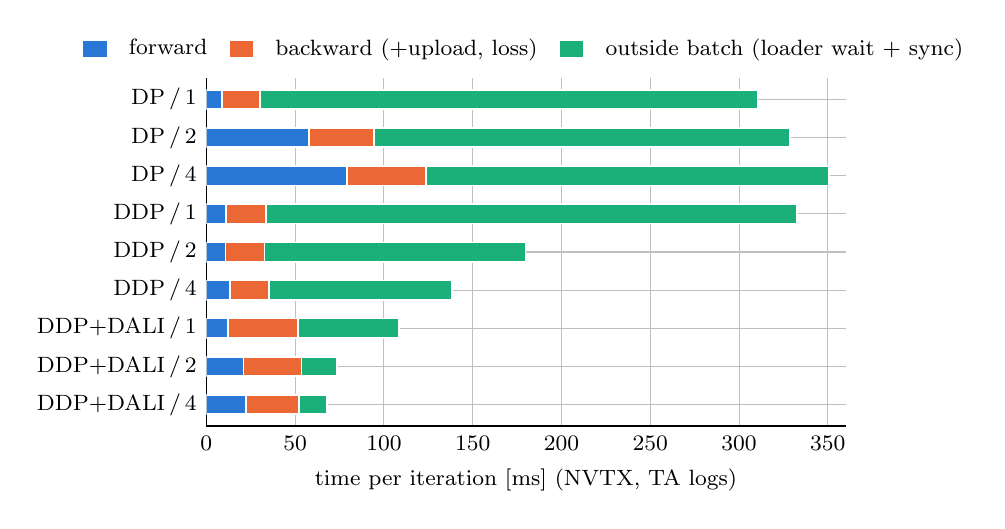
\begin{tikzpicture}
\begin{axis}[
  xbar stacked, bar width=7pt, width=0.80\linewidth, height=6.0cm,
  xmin=0, xmax=360, xlabel={\LblIterAxis},
  symbolic y coords={DALI-4,DALI-2,DALI-1,DDP-4,DDP-2,DDP-1,DP-4,DP-2,DP-1},
  ytick={DALI-4,DALI-2,DALI-1,DDP-4,DDP-2,DDP-1,DP-4,DP-2,DP-1},
  yticklabels={DDP+DALI\,/\,4,DDP+DALI\,/\,2,DDP+DALI\,/\,1,DDP\,/\,4,DDP\,/\,2,DDP\,/\,1,DP\,/\,4,DP\,/\,2,DP\,/\,1},
  y tick label style={font=\footnotesize}, x tick label style={font=\footnotesize}, xlabel style={font=\footnotesize},
  axis x line*=bottom, axis y line*=left, xmajorgrids, grid style={grid},
  major tick length=0pt, enlarge y limits=0.07,
  legend style={font=\footnotesize, draw=none, at={(0.5,1.02)}, anchor=south, legend columns=3, column sep=6pt},
  legend image code/.code={\draw[#1, draw=none] (0cm,-0.1cm) rectangle (0.3cm,0.1cm);},
  every axis plot/.append style={draw=white, line width=0.6pt},
]
\addplot[fill=s1] coordinates {(8.8,DP-1) (57.9,DP-2) (79.4,DP-4) (11.0,DDP-1) (10.8,DDP-2) (13.3,DDP-4) (12.2,DALI-1) (21.0,DALI-2) (22.4,DALI-4)};
\addplot[fill=s2] coordinates {(21.6,DP-1) (36.7,DP-2) (44.4,DP-4) (22.7,DDP-1) (22.0,DDP-2) (22.0,DDP-4) (39.4,DALI-1) (32.5,DALI-2) (29.7,DALI-4)};
\addplot[fill=s3] coordinates {(280,DP-1) (234,DP-2) (227,DP-4) (299,DDP-1) (147,DDP-2) (103,DDP-4) (57,DALI-1) (20,DALI-2) (16,DALI-4)};
\legend{{\LblFwd}, {\LblBwd}, {\LblOut}}
\end{axis}
\end{tikzpicture}

\caption{Per-iteration breakdown from the NVTX rows (mode\,/\,\#GPU). Values are in Table~\ref{tab:nvtx}.}
\label{fig:nvtx}
\end{figure}

\begin{table}[h]
\centering\small
\caption{NVTX breakdown and GPU metrics (TA logs, mean over GPUs). Busy = compute-kernel busy time over the epoch.}
\label{tab:nvtx}
% NVTX breakdown and GPU metrics (TA logs, mean over GPUs). Values from report/results.json
\setlength{\tabcolsep}{3.8pt}
\begin{tabular}{@{}llrrrrrrrrrr@{}}
\toprule
& & \multicolumn{5}{c}{NVTX [ms / iter]} & \multicolumn{3}{c}{GPU [\%]} & \multicolumn{2}{c}{per GPU} \\
\cmidrule(lr){3-7}\cmidrule(lr){8-10}\cmidrule(l){11-12}
Mode & GPU & epoch [s] & iter & fwd & bwd & outside & SMs act. & DRAM R/W & busy & kernel ms/it & NCCL [s] \\
\midrule
\multirow{3}{*}{DP}       & 1 & 30.4 & 310 &  8.8 & 20.9 & 280 & 28.0 & 9.1 / 5.3 & 31.1 & 96.4 & -- \\
                          & 2 & 32.2 & 328 & 57.9 & 35.9 & 234 & 14.1 & 4.4 / 2.6 & 15.9 & 52.3 & 0.98 \\
                          & 4 & 34.4 & 351 & 79.4 & 43.1 & 227 &  6.8 & 2.2 / 1.3 &  7.8 & 27.5 & 2.50 \\
\midrule
\multirow{3}{*}{DDP}      & 1 & 32.6 & 333 & 11.0 & 22.1 & 299 & 26.3 & 8.5 / 5.0 & 29.2 & 97.0 & -- \\
                          & 2 & 17.7 & 180 & 10.8 & 21.4 & 147 & 24.8 & 8.0 / 4.8 & 28.3 & 51.1 & 2.18 \\
                          & 4 & 13.6 & 138 & 13.3 & 21.3 & 103 & 17.0 & 5.5 / 3.5 & 22.4 & 31.0 & 4.01 \\
\midrule
\multirow{3}{*}{DDP+DALI} & 1 & 10.6 & 109 & 12.2 & 38.7 &  57 & 82.0 & 25.7 / 15.1 & 91.1 & 99.0 & -- \\
                          & 2 &  7.2 &  74 & 21.0 & 31.6 &  20 & 61.2 & 19.3 / 11.6 & 70.2 & 51.7 & 1.81 \\
                          & 4 &  6.7 &  69 & 22.4 & 28.9 &  16 & 34.1 & 11.0 / 7.0 & 45.9 & 31.5 & 3.44 \\
\bottomrule
\end{tabular}

\end{table}

\begin{figure}[h]
\centering
% SMs Active and epoch time vs. #GPU (TA logs). Labels: \LblGPU, \LblSMs, \LblEpoch
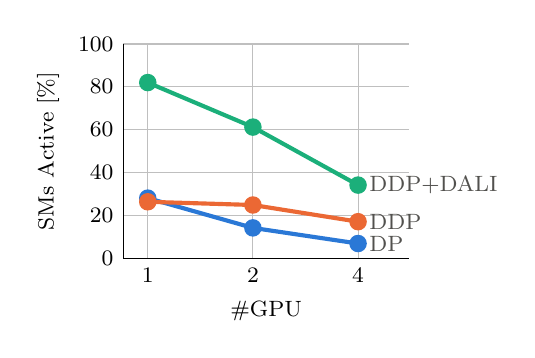
\begin{tikzpicture}
\begin{axis}[
  width=0.43\linewidth, height=4.3cm, xmode=log, log basis x=2,
  xtick={1,2,4}, xticklabels={1,2,4}, xmin=0.85, xmax=5.6, ymin=0, ymax=100,
  xlabel={\LblGPU}, ylabel={\LblSMs},
  tick label style={font=\footnotesize}, label style={font=\footnotesize},
  axis x line*=bottom, axis y line*=left, ymajorgrids, grid style={grid}, major tick length=0pt,
  every axis plot/.append style={line width=1.5pt, mark size=2.4pt}, clip=false,
]
\addplot[s1, mark=*] coordinates {(1,28.0) (2,14.1) (4,6.8)} node[right, font=\footnotesize, text=ink2] {DP};
\addplot[s2, mark=*] coordinates {(1,26.3) (2,24.8) (4,17.0)} node[right, font=\footnotesize, text=ink2] {DDP};
\addplot[s3, mark=*] coordinates {(1,82.0) (2,61.2) (4,34.1)} node[right, font=\footnotesize, text=ink2] {DDP+DALI};
\end{axis}
\end{tikzpicture}\hfill
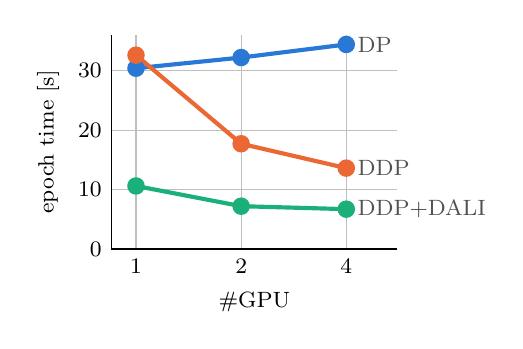
\begin{tikzpicture}
\begin{axis}[
  width=0.43\linewidth, height=4.3cm, xmode=log, log basis x=2,
  xtick={1,2,4}, xticklabels={1,2,4}, xmin=0.85, xmax=5.6, ymin=0, ymax=36,
  xlabel={\LblGPU}, ylabel={\LblEpoch},
  tick label style={font=\footnotesize}, label style={font=\footnotesize},
  axis x line*=bottom, axis y line*=left, ymajorgrids, grid style={grid}, major tick length=0pt,
  every axis plot/.append style={line width=1.5pt, mark size=2.4pt}, clip=false,
]
\addplot[s1, mark=*] coordinates {(1,30.4) (2,32.2) (4,34.4)} node[right, font=\footnotesize, text=ink2] {DP};
\addplot[s2, mark=*] coordinates {(1,32.6) (2,17.7) (4,13.6)} node[right, font=\footnotesize, text=ink2] {DDP};
\addplot[s3, mark=*] coordinates {(1,10.6) (2,7.2) (4,6.7)} node[right, font=\footnotesize, text=ink2] {DDP+DALI};
\end{axis}
\end{tikzpicture}

\caption{GPU utilization (SMs Active, left) and epoch time (right) vs.\ number of GPUs (TA logs, values in Table~\ref{tab:nvtx}).}
\label{fig:scaling}
\end{figure}

\begin{table}[h]
\centering\small
\caption{Our Vast.ai runs (nvidia-smi sampled every 200\,ms inside the epoch; memory = peak allocated / nvidia-smi max, per GPU).}
\label{tab:ours}
% Our Vast.ai runs. Values from report/results.json and logs/nvidia_smi.csv
\footnotesize\setlength{\tabcolsep}{4pt}
\begin{tabular}{@{}llrrrrrrr@{}}
\toprule
Mode & GPU & epoch [s] & iter [ms] & outside [ms] & busy [\%] & smi GPU/mem [\%] & mem. [MiB] & H$\to$D [MiB] \\
\midrule
DP       & 1 & 27.8 & 284 & 259 & 37.9 & 40 / 21 & 3544 / 3854 & 586 \\
DP       & 2 & 33.4 & 341 & 261 & 14.9 & 44 / 8  & 1939 / 2312 & 881 \\
DDP      & 1 & 27.7 & 282 & 252 & 38.2 & 37 / 18 & 3662 / 4022 & 586 \\
DDP      & 2 & 18.2 & 186 & 158 & 38.4 & 48 / 15 & 1957 / 2378 & 586 \\
DDP+DALI & 1 & 11.7 & 119 &  90 & 93.9 & 92 / 45 & 4086 / 4552 & 158 \\
DDP+DALI & 2 &  9.7 &  99 &  65 & 74.8 & 90 / 28 & 2389 / 2748 & 158 \\
\bottomrule
\end{tabular}

\end{table}

\section{Analysis: how and why GPU/memory utilization changes}

\textbf{Baseline (1 GPU).} With the torchvision loader (\texttt{num\_workers=0}), the \emph{outside-batch} time is 280--300\,ms of a
310--333\,ms iteration. Our logs confirm that this is data loading: the loader's own \texttt{Data} timer is 0.17\,s per iteration. PNG decode and augmentation of
512 images run on one CPU thread, while the GPU needs only $\approx$97\,ms of kernels per iteration. The GPU is therefore idle about 70\% of the time
(SMs Active 26--28\%, DRAM read 9\%). Both DP and DDP start from this CPU-bound point.

\textbf{DP gets slower with more GPUs.} Kernel time per GPU halves (96$\rightarrow$52$\rightarrow$28\,ms), but utilization falls roughly as $1/N$
(SMs Active 28$\rightarrow$14$\rightarrow$7\%, DRAM read 9$\rightarrow$4$\rightarrow$2\%) and the epoch grows (30.4$\rightarrow$34.4\,s). Two reasons:
(i) a single process still loads all 512 images per iteration, so the outside-batch time stays at 227--280\,ms and extra GPUs only wait longer.
(ii) The DP work inside the batch grows: \texttt{forward} goes from 8.8 to 79.4\,ms, because every iteration scatters the input, replicates the
parameters (\texttt{ncclBroadcast}), runs the replicas from Python threads under the GIL, and gathers the outputs on GPU\,0; \texttt{backward} goes from 21 to 43\,ms
because of the gradient \texttt{ncclReduce}. The input also crosses PCIe twice: H$\to$D grows from 586 to 881/1029\,MiB and D$\to$H from 0 to
295/442\,MiB, exactly $(N{-}1)/N$ of the batch, because GPU\,0 scatters through host memory. This is the communication overhead the TAs warned
about; it grows with $N$ while the useful work per GPU shrinks. Memory per GPU also halves (3544$\rightarrow$1939\,MiB allocated), since each replica
holds only $512/N$ activations.

\textbf{DDP scales with the number of processes.} DDP runs one process per GPU, so each loads only its $512/N$ shard in parallel. The outside-batch
time falls 299$\rightarrow$147$\rightarrow$103\,ms and the epoch 32.6$\rightarrow$17.7$\rightarrow$13.6\,s (2.4$\times$ on 4 GPUs). The batch range stays
at $\approx$33\,ms. Parameters are synchronized once (\texttt{Sync model parameters}); per step only the small BatchNorm buffers are broadcast (all
\texttt{ncclBroadcast} calls fall inside \texttt{forward}), with no input scatter or model replication as in DP. Gradients are all-reduced in 2--3 buckets
that overlap with \texttt{backward}: 544 of the 1368 \texttt{ncclAllReduce} calls (2 GPUs) fall inside \texttt{backward}, and most of the rest are the
per-step metric \texttt{reduce\_tensor} outside the batch range. As a result, utilization per GPU is
roughly kept at 2 GPUs (SMs 26$\rightarrow$25\%, DRAM 8.5$\rightarrow$8.0\%). At 4 GPUs it drops to 17\% because the per-GPU compute (31\,ms) shrinks faster than the loader
time, and NCCL kernels (4.0\,s per GPU) spend more time waiting for the slowest rank. The bucket copies show up as 4.2\,GiB of D$\to$D traffic per GPU per epoch.
Peak memory per GPU is the same as DP's (1957\,MiB on 2 GPUs) and balanced across ranks.

\textbf{DALI removes the loader bottleneck.} DALI prefetches batches and runs crop/flip/normalize/cutout on the GPU, overlapping them with training.
On 1 GPU the outside-batch time falls from 299 to 57\,ms and the epoch from 32.6 to 10.6\,s (3.1$\times$). The GPU becomes busy
(SMs Active 82\%, compute busy 91\%, nvidia-smi 92\%) and memory bandwidth use triples (DRAM read 26\%, nvidia-smi memory util 45\% vs.\ 18\%). Most of the remaining
outside-batch time is now \texttt{.item()} waiting for queued kernels, not data. H$\to$D traffic drops 3.7$\times$ (586$\rightarrow$158--172\,MiB), because uint8
images are uploaded instead of normalized float32 tensors. The costs: the pipeline build makes \texttt{Set data loader} 3.3\,s instead of 1.0\,s, and DALI buffers use
$\approx$430\,MiB more GPU memory (4086 vs.\ 3662\,MiB). Multi-GPU scaling now hits another limit. Per-GPU kernel time falls to 31\,ms on 4 GPUs, but the CPU-side batch range
stays at $\approx$52\,ms, so launching ResNet-18's kernels for a small batch of 128 dominates. SMs Active drops to 61\% (2 GPUs) and 34\% (4 GPUs), and the epoch improves only 10.6$\rightarrow$7.2$\rightarrow$6.7\,s.

\textbf{Notes.} (1) nvidia-smi's \emph{GPU util} counts any running kernel, including NCCL kernels waiting for peers. For our DP 2-GPU run it reports 44\%
while compute kernels are busy only 15\%, so we use SMs Active and compute-busy time. (2) The TA logs report \emph{GPU Active} = 100\% on some GPUs with the same
SMs Active as the others, so we do not use that metric. (3) Our instance has no GPU peer-to-peer access, and its per-GPU kernel time for DDP on 2 GPUs is higher (71 vs.\ 51\,ms).
The trends and the ranking DP $<$ DDP $<$ DDP+DALI are the same as in the TA logs.

\textbf{Conclusion.} DP is limited by a single-process data loader and by per-iteration scatter/replicate/gather, so adding GPUs lowers
utilization and slows training. DDP parallelizes loading across processes and overlaps gradient all-reduce with backward, which gives near-linear speedup
while loading dominates. DALI moves augmentation to the GPU and prefetches asynchronously, which raises GPU and memory-bandwidth utilization to 80--90\%
on one GPU. After that, the next bottleneck is CPU kernel-launch overhead for small per-GPU batches.

\section{Final loss and accuracy}

After one epoch, all runs reach a similar train loss (1.74--1.81), but the test accuracy ranges from 46.6\% to 55.2\%
(DP 55.2/49.2\%, DDP 48.8/50.5\%, DDP+DALI 46.6/47.7\% on 1/2 GPUs). In expectation the three modes run the same SGD:
same model, optimizer, augmentation and global batch 512, and DDP's all-reduce of two 256-sample means equals DP's 512-sample mean.
The spread is mostly run-to-run noise: \texttt{--seed} is never applied (initial weights, data order and augmentation differ per run),
training is a single warm-up epoch at lr 0.04, and re-running DDP on 2 GPUs gave 50.5\% and 48.5\%. Smaller systematic
differences are BatchNorm statistics over 256 instead of 512 samples per GPU (no SyncBN), different sampling orders, and, for DALI, the
cutout placement and possibly the reader's buffer-based shuffle over a class-sorted file list (unverified; DALI was 1--2\,pt lower in all
three runs). DP's logged loss looks $\approx$500$\times$ smaller only because \texttt{DP/train.py} divides the mean loss by the batch size again.

\end{document}
